% !TeX encoding = UTF-8

\chapter{IMPLEMENTAÇÃO DAS TÉCNICAS}\label{ch:implementacao}

Este capítulo tem como finalidade apresentar, com um maior nível de detalhamento as técnicas utilizadas neste trabalho, com o objetivo de se atingir as metas propostas já descritas na \autoref{sec:objetivos}.

\section{COLETA DE DADOS}
Uma característica comentada anteriormente ....

As primeiras linhas mostradas no \autoref{coleta-script} servem para ...

\codigoPython
\lstinputlisting[language=Python, label=coleta-script, caption=\textit{Script} coletar-hashtags.py]{src/coletar-hashtags.py}

...


O comando \textit{stdout} permite redirecionar a saída do código anterior, no caso a execução do \textit{script} coletar-hashtags.py, para um novo arquivo ou um arquivo já existente, conforme ilustrado pela \autoref{exec-coleta}.

\begin{figure}[h]
	\centering
	\fbox{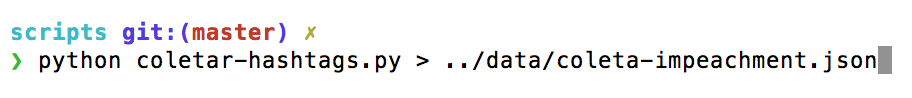
\includegraphics[width=0.95\textwidth]{execucao-script}}
	\caption{Execução do \textit{script} para coleta de dados}
	\fonte{Autor}
	\label{exec-coleta}
\end{figure}

...


\section{ANÁLISE DE DADOS}
Após a coleta dos dados foi gerado, então, um arquivo ....

